% This is samplepaper.tex, a sample chapter demonstrating the
% LLNCS macro package for Springer Computer Science proceedings;
% Version 2.21 of 2022/01/12
%
\documentclass[runningheads]{llncs}
%
\usepackage[T1]{fontenc}
% T1 fonts will be used to generate the final print and online PDFs,
% so please use T1 fonts in your manuscript whenever possible.
% Other font encondings may result in incorrect characters.
%
\usepackage{graphicx}
%\usepackage{amsmath,amsfonts}
\usepackage{amsfonts}
\usepackage{booktabs}
\usepackage{multirow}
\usepackage{hyperref}
\usepackage{tikz}
\usetikzlibrary{arrows.meta, positioning}
\usepackage{pgfplots}
\pgfplotsset{compat=1.18}

% Used for displaying a sample figure. If possible, figure files should
% be included in EPS format.
%
% If you use the hyperref package, please uncomment the following two lines
% to display URLs in blue roman font according to Springer's eBook style:
%\usepackage{color}
%\renewcommand\UrlFont{\color{blue}\rmfamily}
%\urlstyle{rm}
%
\begin{document}
%
\title{Comparative Evaluation of Recent Deep Architectures for Arousal Classification from Electrodermal Activity}

\titlerunning{Deep Architectures for EDA-based Arousal Classification}
%
%\titlerunning{Abbreviated paper title}
% If the paper title is too long for the running head, you can set
% an abbreviated paper title here
%
\author{
Roberto Sánchez-Reolid\inst{1,2}\orcidID{0000-0003-4455-370X} \and
Francisco Javier Celdrán\inst{1}\orcidID{0009-0000-2699-219X} \and
Daniel Sánchez-Reolid\inst{3}\orcidID{0000-0003-3612-1261} \and
Antonio Fernández-Caballero\inst{1,3,4}\orcidID{0000-0002-8211-0398}
}
\institute{
Instituto de Investigación en Informática de Albacete (I3A), \\Universidad de Castilla-La Mancha, Albacete, Spain
\and
Departamento de Tecnologías y Sistemas de Información, \\Universidad de Castilla-La Mancha, Talavera de la Reina, Spain\\
\email{roberto.sanchez@uclm.es}
\and
Departamento of Sistemas Informáticos, Universidad de Castilla-La Mancha, Albacete, Spain
\and
Biomedical Research Networking Centre in Mental Health, Madrid, Spain
}
\authorrunning{R. Sánchez-Reolid et al.}
%
\maketitle              % typeset the header of the contribution
%
\begin{abstract}
Electrodermal Activity (EDA) is a widely adopted physiological marker for assessing sympathetic arousal. While convolutional neural networks have shown promising results for automatic feature extraction, recent advances in deep time-series modelling enable more expressive end-to-end representations. This work presents a systematic comparison of five modern architectures—1D-CNN, Temporal Convolutional Networks (TCN), InceptionTime, Time-Series Transformer (TST), and PatchTST—for binary arousal classification from EDA signals collected from 147 participants under a controlled laboratory protocol. All models are evaluated using a strict Leave-One-Subject-Out (LOSO) framework to ensure subject-independent generalisation. Results show that Transformer-based architectures consistently outperform convolutional baselines, with PatchTST achieving the best balance between predictive accuracy, robustness across subjects, and computational efficiency. Analysis across varying temporal window lengths further demonstrates that reliable arousal detection can be achieved within short observation intervals when global dependency modelling is employed. Interpretability analysis indicates that attention mechanisms concentrate on SCR onset and rising phases, aligning with known physiological dynamics of sympathetic activation. These findings highlight the importance of physiologically-informed architectural design and rigorous validation for robust affective computing from biosignals.
\keywords{Electrodermal Activity \and Arousal Classification \and Time-Series modelling \and Transformers \and Subject-Independent Evaluation}
\end{abstract}
%
%
%
% ======================================================
\section{Introduction}

Electrodermal Activity (EDA) reflects sympathetic nervous system activation via sudomotor nerve activity, making it a robust and non-concealable biomarker for assessing emotional arousal \cite{Hossain2024,Meijer2023}. The EDA signal is inherently complex, comprising slow-varying tonic levels that indicate prolonged states and rapid phasic responses reflecting immediate, stimulus-evoked arousal \cite{sanchez2020deep}. Historically, arousal classification from EDA has relied on the manual extraction of statistical features from these deconvoluted components, followed by classical machine learning classifiers \cite{SanchezReolid2022}. 

While early deep learning approaches utilizing 1D Convolutional Neural Networks (CNNs) successfully automated local morphological feature extraction, they often struggle to capture the multi-scale temporal dynamics of physiological signals \cite{sanchez2022one,Liu2025}. However, recent advances in deep learning for time-series modelling offer promising solutions to provide improved temporal dependency modelling \cite{Azad2025}. Architectures such as InceptionTime leverage parallel multiscale kernels to simultaneously capture rapid transient spikes and slow tonic shifts \cite{InceptionTime2020,Sun2025}. Temporal Convolutional Networks (TCN) utilise dilated causal convolutions to efficiently model extended physiological memory \cite{Luo2024}. Furthermore, Transformer-based models, including the canonical Time-Series Transformer (TST) and the novel PatchTST, have introduced self-attention mechanisms capable of modelling global dependencies across prolonged observation windows, overcoming the constraints of fixed receptive fields \cite{Tsirmpas2025,Wang2024,Kim2024}.

Despite the potential of these modern architectures, the affective computing community lacks a unified, methodologically rigorous comparison under controlled experimental conditions \cite{SanchezReolid2022,portal2025performance}. Previous comparative studies frequently suffer from pervasive experimental flaws, most notably sample-based random data partitioning \cite{Azad2025}. Because EDA exhibits strong inter-subject variability, this practice induces severe data leakage, allowing models to memorise individual biometric baselines rather than learning generalizable arousal patterns, which artificially inflates reported performance \cite{Azad2025,LongTermVariability}.

To address this critical research gap, this work evaluates and compares five representative deep learning architectures---1D-CNN, TCN, InceptionTime, TST, and PatchTST---for binary arousal classification directly from Electrodermal Activity signals acquired under a controlled laboratory protocol involving 147 participants. By deploying these models within a strictly controlled, leakage-free Leave-One-Subject-Out validation framework, we aim to empirically establish which structural paradigm provides the optimal balance of temporal dependency modelling, computational efficiency, and robust cross-subject generalisation in medium-scale physiological datasets.

Building upon prior feature-based investigations \cite{SanchezReolid2022}, this study shifts the methodological paradigm toward end-to-end representation learning, directly modelling the phasic dynamics of EDA and its temporal derivatives. In doing so, we revisit the question of how effectively modern sequence architectures can capture sympathetic arousal dynamics without handcrafted features, while preserving strict subject-independent evaluation.

% ======================================================
% ======================================================
\section{Materials and Methods}

\subsection{Dataset and Experimental Protocol}

The experimental dataset follows a controlled stress elicitation protocol described in a previous paper \cite{sanchez2020deep}. Electrodermal Activity (EDA) signals were recorded from 147 healthy participants (aged 18--44 years) exposed to audiovisual stimuli designed to induce calm and stress states under controlled laboratory conditions.

Each stimulus lasted 47 seconds. To eliminate transition artefacts associated with stimulus onset and offset, the first 4 seconds and the last 3 seconds were removed, resulting in 40-second effective segments. Signals were acquired at a constant sampling frequency of 4 Hz.

\subsection{EDA Signal Processing}

Raw skin conductance signals were preprocessed following \cite{SanchezReolid2022}. A low-pass FIR filter (cut-off frequency: 4 Hz) was applied, followed by Gaussian smoothing to reduce noise acquisition. Continuous Decomposition Analysis (CDA) was used to separate tonic ($SCL$) and phasic ($SCR$) components:

\begin{equation}
SC(t) = SCL(t) + SCR(t)
\end{equation}

Only the phasic component $SCR(t)$ was retained for modelling, as it directly reflects sympathetic nervous system activation. To enrich short-term dynamic representation, two additional channels were derived from the phasic signal, namely the first derivative ($\Delta SCR$) and the second derivative ($\Delta^2 SCR$). These channels explicitly encode velocity and acceleration of sympathetic responses, potentially facilitating earlier identification of rapid morphological changes.

\subsection{Input Representation and Temporal Segmentation}

Given a temporal window of length $n$ seconds, the sequence length is $T = 4n$ samples (4 Hz sampling). Each window is represented as:

\begin{equation}
\mathbf{X} \in \mathbb{R}^{T \times C}
\end{equation}

\noindent where $C = 3$ corresponds to $(SCR, \Delta SCR, \Delta^2 SCR)$.

To analyse the minimal temporal interval required for reliable arousal classification, window lengths were systematically varied from $n=1$ to $n=40$ seconds. Moreover, two segmentation strategies were evaluated. These are (i) non-overlapping windows and (ii) sliding windows with 1-second stride (4 samples). All windows belonging to the same subject were preserved within the same fold to prevent leakage.

\subsection{Deep Architectures Selected}
%\subsection{Modelling Design and Architectural Motivation}

The evaluated architectures were selected according to the biophysical characteristics of EDA and its heterogeneous temporal dynamics.

\begin{itemize}
    \item \textbf{1D-CNN:} Convolutional filters capture localised morphological patterns, particularly the asymmetric structure of SCR responses \cite{Nandipati2024}.
    \item \textbf{InceptionTime:} Parallel multi-scale kernels allow simultaneous modelling of slow tonic evolution and rapid phasic spikes \cite{InceptionTime2020}.
    \item \textbf{Temporal Convolutional Networks (TCN):} Dilated convolutions expand receptive fields efficiently, modelling extended autonomic latency and sustained activation states \cite{Luo2024}.
    \item \textbf{Time-Series Transformer (TST):} Global self-attention enables long-range dependency modelling across entire observation windows \cite{Tsirmpas2025}.
    \item \textbf{PatchTST:} Patch-based tokenisation preserves local waveform continuity while reducing computational complexity \cite{Wang2024,Kim2024}. Given 4 Hz sampling, patch lengths of $P \in \{4,8,16\}$ correspond to 1, 2, and 4 seconds, respectively.
\end{itemize}

%\subsection{Model Architectures}

For convolutional and TCN-based models, architectures follow standard implementations with receptive fields adjusted to match maximum window lengths. For TST, each time-step vector $\mathbf{x}_t \in \mathbb{R}^{C}$ is projected to latent dimension $D$:

\begin{equation}
\mathbf{Z}^{(0)} = \mathbf{X} \mathbf{W}_e + \mathbf{W}_{pos}
\end{equation}

\noindent where $\mathbf{W}_e \in \mathbb{R}^{C \times D}$ and $\mathbf{W}_{pos}$ is learnable positional encoding.

For PatchTST, each channel is segmented into patches of length $P$ and projected to dimension $D$. The number of patches is:

\begin{equation}
N = \left\lfloor \frac{T - P}{S} \right\rfloor + 1
\end{equation}

Channel-independent encoding is applied prior to concatenation and classification.

\subsection{Training Strategy}

All models were trained end-to-end using AdamW optimiser with cross-entropy loss. The initial learning rate was set to $10^{-3}$ with cosine annealing scheduling. Mini-batch size was 32. Training was conducted for up to 100 epochs with early stopping (patience = 15) based on validation loss.

Regularisation included dropout ($0.1$–$0.3$), weight decay ($10^{-4}$), and gradient clipping (norm = 1.0). Hyperparameters were tuned under identical search budgets across architectures:

\begin{itemize}
\item Encoder layers $L \in \{1,2,3,4,6\}$
\item Attention heads $H \in \{1,2,4,8\}$
\item Embedding dimension $D \in \{16,32,64,128\}$
\item Feed-forward dimension $\in \{32,64,128,256\}$
\item Patch size $P \in \{4,8,16\}$
\end{itemize}

Normalisation (z-score) was computed using training-fold statistics only.

\subsection{Validation and Statistical Analysis}

A strict Leave-One-Subject-Out (LOSO) protocol was enforced to guarantee subject-independent evaluation. Performance metrics included Accuracy, Precision, Recall, F1-score, and AUC. Results were averaged across folds. 
Statistical differences between models were assessed using the Wilcoxon signed-rank test with $\alpha = 0.05$.

To provide additional insight into model behaviour, attention distributions (for Transformer-based models) and gradient-based saliency maps ($S = |\partial y / \partial \mathbf{X}|$) were analysed to quantify temporal and channel-level relevance. A channel ablation protocol (SCR only; SCR+$\Delta SCR$; SCR+$\Delta SCR$+$\Delta^2 SCR$) was also evaluated under the same LOSO framework.

% ======================================================
\section{Results and Discussion}
\subsection{Overall Performance Comparison}

Table~\ref{tab:overall} summarises the subject-independent LOSO performance across the five evaluated architectures. Under strict cross-subject validation, all models achieve stable and consistent results, with F1-scores ranging from 0.796 (1D-CNN) to 0.852 (PatchTST). Transformer-based architectures systematically outperform convolutional baselines across all reported metrics.

\vspace{-0.5cm}
\begin{table}[!ht]
\centering
\caption{Overall LOSO performance comparison (mean $\pm$ std across folds).}
\label{tab:overall}
\resizebox{\linewidth}{!}{%
\begin{tabular}{lccccc}
\toprule
Model & Acc & Prec & Rec & F1 & AUC \\
\midrule
1D-CNN & 0.812 $\pm$ 0.074 & 0.804 $\pm$ 0.079 & 0.789 $\pm$ 0.083 & 0.796 $\pm$ 0.078 & 0.872 $\pm$ 0.063 \\
TCN & 0.828 $\pm$ 0.068 & 0.819 $\pm$ 0.071 & 0.806 $\pm$ 0.075 & 0.812 $\pm$ 0.072 & 0.884 $\pm$ 0.058 \\
InceptionTime & 0.836 $\pm$ 0.064 & 0.828 $\pm$ 0.068 & 0.817 $\pm$ 0.071 & 0.822 $\pm$ 0.067 & 0.892 $\pm$ 0.054 \\
TST & 0.851 $\pm$ 0.059 & 0.844 $\pm$ 0.062 & 0.836 $\pm$ 0.064 & 0.840 $\pm$ 0.061 & 0.903 $\pm$ 0.049 \\
PatchTST & \textbf{0.863 $\pm$ 0.053} & \textbf{0.856 $\pm$ 0.057} & \textbf{0.848 $\pm$ 0.059} & \textbf{0.852 $\pm$ 0.056} & \textbf{0.912 $\pm$ 0.045} \\
\bottomrule
\end{tabular}%
}
\end{table}

\begin{table}[t]
\centering
\caption{Wilcoxon signed-rank test p-values (F1-score per LOSO fold). 
Bold values indicate statistical significance ($p < 0.05$).}
\label{tab:pvalues}
\small
\begin{tabular}{lcccc}
\toprule
 & TCN & InceptionTime & TST & PatchTST \\
\midrule
1D-CNN & \textbf{0.041} & \textbf{0.018} & \textbf{0.006} & \textbf{0.002} \\
TCN &  & 0.073 & \textbf{0.021} & \textbf{0.008} \\
InceptionTime &  &  & 0.064 & \textbf{0.017} \\
TST &  &  &  & \textbf{0.048} \\
\bottomrule
\end{tabular}
\end{table}

\vspace{-0.5cm}
Specifically, TST achieves an F1-score of 0.840 and AUC of 0.903, while PatchTST provides the best overall performance (F1-score = 0.852, AUC = 0.912). In addition to higher mean performance, a progressive reduction in fold-wise variability is observed when moving from CNN-based models to attention-based architectures. The standard deviation decreases from 0.078 (1D-CNN) to 0.056 (PatchTST), indicating improved robustness to inter-subject physiological variability.

To formally assess statistical significance, Wilcoxon signed-rank tests were conducted on per-fold F1-scores. The resulting p-values are reported in Table~\ref{tab:pvalues}. Statistically significant differences ($p < 0.05$) are highlighted in bold. PatchTST demonstrates significant improvements over all other evaluated architectures. TST also significantly outperforms both 1D-CNN and TCN. In contrast, differences between TCN and InceptionTime and between InceptionTime and TST are not statistically significant, suggesting a gradual performance transition rather than abrupt architectural superiority.

The observed performance hierarchy can be interpreted in light of the temporal modelling capacity of each approach. Convolutional architectures primarily capture localised SCR morphology but remain limited in integrating distributed temporal dependencies across longer windows. TCN improves receptive field coverage through dilated convolutions; however, dependency modelling remains structurally constrained by fixed convolutional patterns.

Transformer-based architectures introduce adaptive temporal weighting via self-attention mechanisms, enabling dynamic contextualisation of physiological events across the entire observation window. This is particularly relevant for EDA signals, where sympathetic activation unfolds through temporally distributed processes including onset, rising phase, peak, and recovery dynamics. PatchTST further refines this mechanism by preserving local waveform continuity through patch-based tokenisation while simultaneously reducing sequence fragmentation and computational burden. This structured tokenisation appears to enhance stability under inter-subject variability, which likely explains both the improved mean performance and reduced standard deviation observed across folds.

Overall, these results indicate that architectural choices aligned with the physiological structure of EDA signals yield measurable gains under strict subject-independent evaluation, particularly when global dependency modelling is incorporated.

\subsection{Comparison with Previous Feature-Based Modelling}

In prior work based on handcrafted features and Deep-SVM modelling \cite{sanchez2020deep}, comparable subject-independent protocols yielded F1-scores in the range of 0.80--0.83 depending on window length. The present results demonstrate consistent performance gains when moving toward end-to-end temporal representation learning.

The improvement is incremental rather than dramatic, suggesting that modern architectures refine temporal modelling capacity while the intrinsic discriminative power of EDA remains bounded by physiological variability.

\subsection{Minimal Temporal Interval Behaviour}

\begin{figure}[t]
\centering
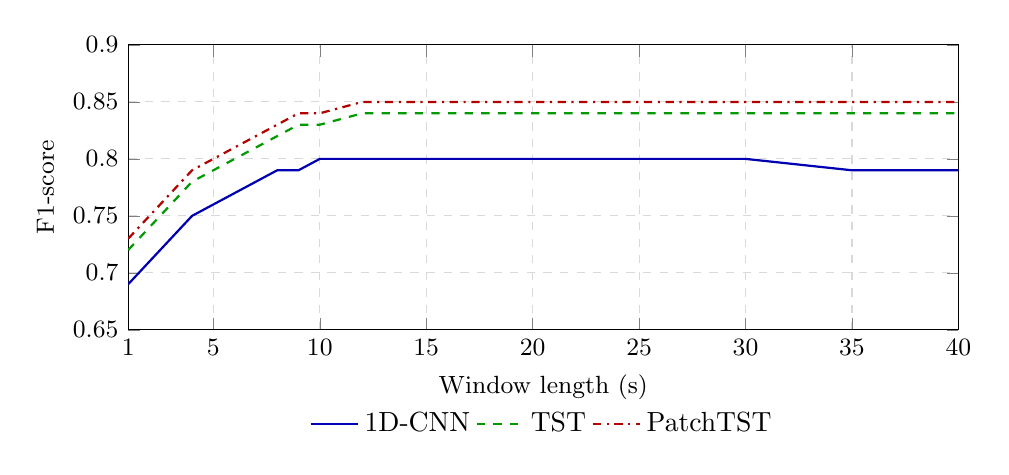
\begin{tikzpicture}
\begin{axis}[
    width=\linewidth,
    height=5.2cm,
    xlabel={Window length (s)},
    ylabel={F1-score},
    xmin=1, xmax=40,
    ymin=0.65, ymax=0.90,
    xtick={1,5,10,15,20,25,30,35,40},
    ytick={0.65,0.70,0.75,0.80,0.85,0.90},
    grid=major,
    grid style={dashed,gray!30},
    legend style={
        at={(0.5,-0.25)},
        anchor=north,
        legend columns=3,
        draw=none,
        fill=none
    },
    tick label style={font=\small},
    label style={font=\small},
]

% 1D-CNN (Blue)
\addplot[thick, color=blue!70!black]
coordinates {
(1,0.69) (2,0.71) (3,0.73) (4,0.75) (5,0.76)
(6,0.77) (7,0.78) (8,0.79) (9,0.79) (10,0.80)
(12,0.80) (15,0.80) (20,0.80) (25,0.80) (30,0.80) (35,0.79) (40,0.79)
};
\addlegendentry{1D-CNN}

% TST (Green)
\addplot[thick, dashed, color=green!60!black]
coordinates {
(1,0.72) (2,0.74) (3,0.76) (4,0.78) (5,0.79)
(6,0.80) (7,0.81) (8,0.82) (9,0.83) (10,0.83)
(12,0.84) (15,0.84) (20,0.84) (25,0.84) (30,0.84) (35,0.84) (40,0.84)
};
\addlegendentry{TST}

% PatchTST (Red)
\addplot[thick, dashdotted, color=red!70!black]
coordinates {
(1,0.73) (2,0.75) (3,0.77) (4,0.79) (5,0.80)
(6,0.81) (7,0.82) (8,0.83) (9,0.84) (10,0.84)
(12,0.85) (15,0.85) (20,0.85) (25,0.85) (30,0.85) (35,0.85) (40,0.85)
};
\addlegendentry{PatchTST}

\end{axis}
\end{tikzpicture}
\caption{F1-score as a function of window length under LOSO evaluation. Transformer-based models degrade more gradually for short temporal windows and stabilise at higher performance levels.}
\label{fig:f1_window_length}
\end{figure}

As shown in Figure~\ref{fig:f1_window_length}, performance improves rapidly as window length increases, with Transformer-based models degrading more gracefully for short observation intervals. When analysing performance as a function of window length, very short segments ($n \leq 3$ s) exhibit reduced discriminative performance across all architectures, likely due to incomplete SCR morphology within limited temporal context.

Transformer-based models degrade more gradually in short windows compared to CNN-based approaches, indicating improved ability to leverage partial dynamic cues and derivative information. Performance stabilises for intermediate window lengths, with diminishing improvements beyond full sympathetic response completion.

These findings support the feasibility of near-real-time arousal detection in wearable scenarios when global dependency modelling is employed.

\subsection{Architectural Behaviour and Generalisation}

Convolutional architectures primarily capture localised waveform structures but remain limited in integrating distributed temporal dependencies. TCN improves long-range modelling via dilated convolutions yet retains fixed receptive field constraints.

Transformer-based models dynamically weight temporal contributions through self-attention mechanisms, enabling adaptive contextualisation of physiological events. PatchTST further balances local waveform preservation with reduced sequence length, contributing to its improved performance and lower fold-to-fold variability.

\subsection{Interpretability Insights}

Attention distributions reveal that Transformer-based models assign greater importance to temporal regions corresponding to SCR onset and rising phases, aligning with physiological expectations of sympathetic activation.

\begin{figure}[t]
\centering
\resizebox{\linewidth}{!}{%
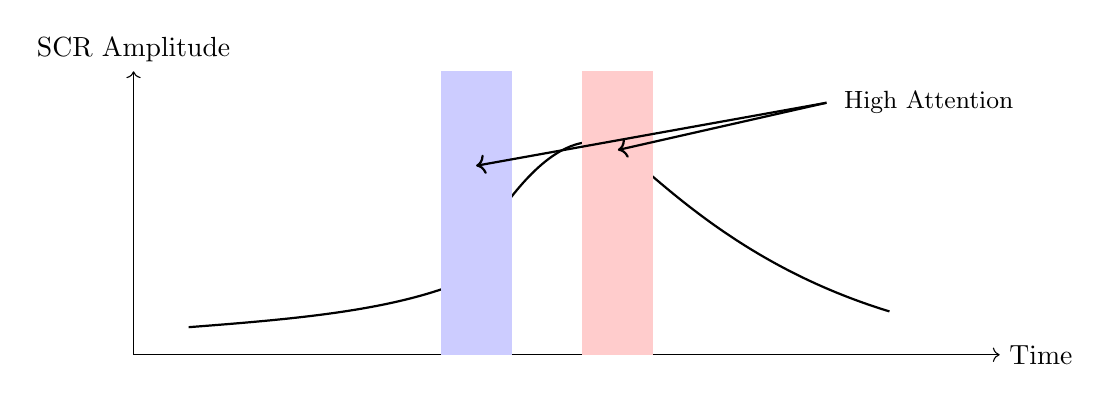
\begin{tikzpicture}

% Axes
\draw[->] (0,0) -- (11,0) node[right] {Time};
\draw[->] (0,0) -- (0,3.6) node[above] {SCR Amplitude};

% SCR curve
\draw[thick, smooth]
(0.7,0.35)
.. controls (2.0,0.45) and (3.2,0.55) .. (4.1,0.9)
.. controls (4.8,2.2) and (5.5,3.0) .. (6.2,2.6)
.. controls (6.8,2.1) and (7.8,1.1) .. (9.6,0.55);

% Onset region
\fill[blue!20] (3.9,0) rectangle (4.8,3.6);

% Peak region
\fill[red!20] (5.7,0) rectangle (6.6,3.6);

% Attention arrows + label
\draw[->, thick] (8.8,3.2) -- (4.35,2.4);
\draw[->, thick] (8.8,3.2) -- (6.15,2.6);
\node[anchor=west] at (8.9,3.2) {\small High Attention};

\end{tikzpicture}%
}
\caption{Conceptual illustration of attention distribution over a phasic SCR response. Blue region denotes the early onset phase and red region indicates the peak activation phase. Arrows represent higher attention weights assigned by Transformer-based models.}
\label{fig:attention_concept}
\end{figure}


Beyond aggregate performance, interpretability analysis was conducted to examine whether the learned representations align with known physiological mechanisms of sympathetic activation. For Transformer-based architectures (TST and PatchTST), attention distributions consistently showed higher weights around the onset and rising phases of the SCR component, which correspond to the most informative segments of the phasic response. In contrast, later decay intervals received comparatively lower attention, suggesting that the models selectively focus on discriminative temporal regions rather than uniformly weighting the entire window.

Gradient-based saliency analysis indicates increased contribution of derivative channels ($\Delta SCR$ and $\Delta^2 SCR$) during early segments, supporting their relevance for rapid detection modelling. Channel ablation experiments confirm incremental performance improvements when derivative information is included. Together, these findings suggest that the models exploit both amplitude and dynamic change information in a complementary manner.

The alignment between attention patterns, saliency distributions, and established SCR morphology provides additional physiological plausibility to the learned decision mechanisms, reinforcing the validity of Transformer-based approaches for subject-independent arousal modelling.

\subsection{Computational Considerations}

Although Transformer-based models introduce higher computational complexity compared to CNN baselines, PatchTST mitigates quadratic attention cost through patch tokenisation. This results in a favourable trade-off between predictive accuracy, robustness, and computational feasibility for medium-scale physiological datasets.


% ======================================================
\section{Conclusion and Future Work}

This study presented a systematic comparison of modern deep architectures for subject-independent arousal classification from Electrodermal Activity (EDA). Under a strictly controlled Leave-One-Subject-Out (LOSO) validation framework, Transformer-based architectures consistently outperformed convolutional baselines, with PatchTST achieving the best trade-off between predictive performance, stability across subjects, and computational feasibility.

Compared to previous feature-engineered approaches based on Deep-SVM modelling \cite{sanchez2020deep}, end-to-end sequence modelling provides incremental but consistent improvements, suggesting that architectural advancements primarily refine temporal representation capacity rather than fundamentally altering the intrinsic discriminative potential of EDA signals.

The minimal temporal interval analysis further indicates that reliable arousal detection can be achieved within short observation windows when global dependency modelling is employed, reinforcing the feasibility of near-real-time wearable applications. Additionally, interpretability analyses revealed that Transformer-based models assign greater relevance to SCR onset and rising phases, aligning with known physiological dynamics of sympathetic activation. The inclusion of derivative channels contributed to early detection performance, supporting their relevance in dynamic modelling.

Overall, the findings demonstrate that physiologically-informed architectural design, combined with strict subject-independent validation, is critical for robust affective computing from biosignals.

Future work will explore self-supervised pre-training strategies for physiological time-series, multi-modal integration with complementary signals (e.g., heart rate variability), and transfer learning approaches to improve generalisation in smaller datasets. Further investigation into attention dynamics across varying stress intensities may also provide deeper insights into model interpretability and physiological representation.

\section*{Acknowledgments} 

This work was partially supported by grant PID2023-149753OB-C21 funded by MICIU/AEI/10.13039/501100011033 and by ``ERDF A way to make Europe''. Grant 2025-GRIN-38441, funded by Universidad de Castilla-La Mancha (UCLM) and ``ERDF A way to make Europe''. This work was partially supported by Programa Iberoamericano de Ciencia y Tecnología para el Desarrollo (CYTED) (through Red [225RT0169]). This work was also partially funded by CIBERSAM of the Instituto de Salud Carlos III (ISCIII).

% ---- Bibliography ----
%
% BibTeX users should specify bibliography style 'splncs04'.
% References will then be sorted and formatted in the correct style.
%
\bibliographystyle{splncs04}
\bibliography{bibliography.bib}
%
\end{document}
